\documentclass[10pt]{article}
\usepackage{graphicx,amssymb, amstext, amsmath, epstopdf, booktabs, verbatim, gensymb, geometry, appendix, natbib, lmodern}
\geometry{letterpaper}
%\usepackage{garamond}

\newcommand*\Title{Rapport de stage de fin d'études}
\newcommand*\cpiType{CPI Template}
\newcommand*\Date{\today}
\newcommand*\Author{Alexandre Léonardi}
\title{Rapport de stage de fin d'études}
\author{Alexandre Léonardi}
\date{\today}
%-----------------------------------------------------------

\usepackage{cpistuff/cpi} % This is what makes your document look like a cpi document.

\begin{document}

\begin{titlepage}
\maketitle
\end{titlepage}

\linespread{1.15} %Set standard document linespacing

\section*{Introduction}
Développement Java et développement d'une solution d'analyse statique de sécurité : ce sont les deux principales branches de mon stage. Il s'agit pour partie de prendre part aux contrats en Java d'Alter Frame, l'entreprise qui m'accueille pour la durée du stage, et d'autre part d'intervenir sur un projet en interne visant à mettre en place une analyse de sécurité systématique des projets Web au-travers de pratiques de CI\cite{ci_wiki}\footnote{Continuous Integration ou intégration continue}. 

Ce sujet a l'avantage d'être ouvert et diversifié. Il me permet d'une part de travailler sur du pur développement et d'autre part de mettre en pratique la composante sécurité de la formation FSI\cite{fsi}\footnote{Fiabilité et sécurité informatique}, tout en découvrant les concepts de CI qui m'étaient jusque là étrangers, ainsi que des technologies qui vont de pair telles que Docker.

En pratique, un troisième pan viendra s'ajouter à mon sujet de stage : un audit technique pour un client d'Alter Frame souhaitant des pistes d'amélioration de son application, notamment en termes de qualité de code. 

À noter que, par discrétion à leur égard, les noms des clients d'Alter Frame ne seront pas mentionnés et seront effacés des captures d'écran que vous trouverez dans ce document. Il en ira de même pour les différents projets.

\pagebreak
\clearpage
\vspace*{\fill}
\begin{center}
\begin{minipage}{.6\textwidth}
\Huge Rapport de synthèse
\end{minipage}
\end{center}
\vfill % equivalent to \vspace{\fill}
\clearpage
\pagebreak

\section{Présentation d'Alter Solutions Engineering} 
Alter Solutions Engineering, et plus particulièrement sa filiale Alter Frame, est l'entreprise qui m'a accueilli pour la durée de mon stage de fin d'études, nous allons donc commencer par la présenter rapidement.

\subsection{Les subdivisions d'Alter Solutions Engineering et leurs secteurs d'activité}
Alter Solutions Engineering est une entreprise relativement jeune : elle a été créée en 2006 et, si elle n'entre plus maintenant dans la catégorie des PME en termes de nombre de collaborateurs, elle reste une structure de petite taille.

Le siège social de l'entreprise se trouve à Versailles et c'est là où travaille l'équipe de développement française dont je fais partie. En pratique, il s'agit de l'équipe de développement d'Alter Frame qui est une entité enfant d'Alter Solutions Engineering (cf. section~\ref{subsec:frame}).

Alter Solutions Engineering est une société de conseil en hautes technologies mais en pratique, elle est composée de trois filières qui ont chacune une spécialité bien distinctes (cf. graphique~\ref{fig:filiales}).
\begin{figure}
  \centering
  \caption{Alter Solutions Engineering et ses filiales}
  \label{fig:filiales}
  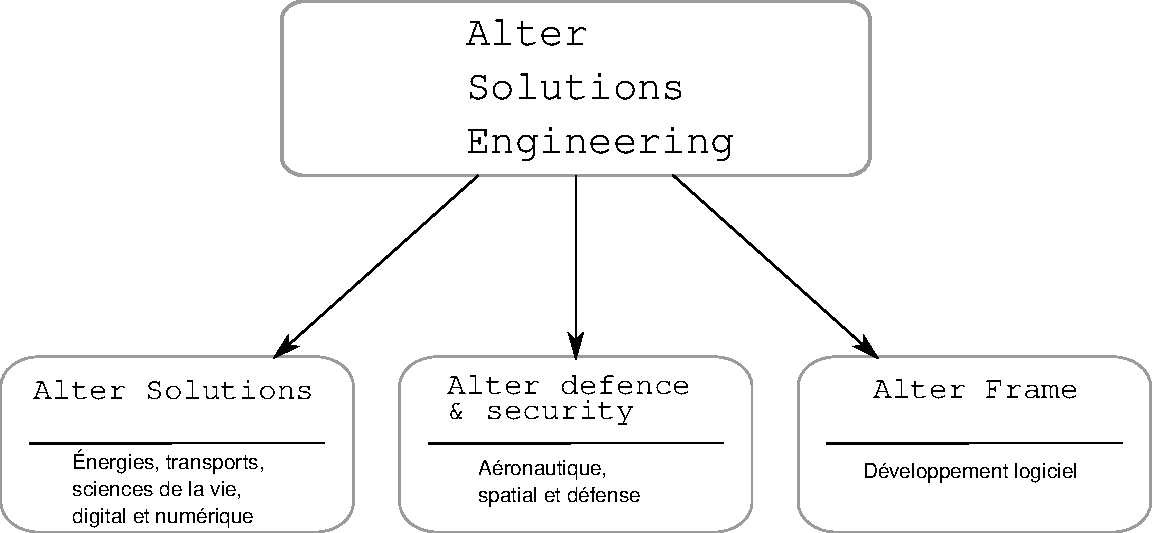
\includegraphics[width=\textwidth]{images/filiales_allinone.pdf}
\end{figure}

\subsubsection{Alter Solutions}
Cette filiale est spécialisée dans le conseil en ingénierie, notamment dans les domaines de l'énergie, des transports, des sciences de la vie, du digital et du numérique.

\subsubsection{Alter defence \& security}
Alter defence est également orientée vers le conseil, mais cette fois plus particulièrement dans l'aéronautique, le sptial et la défense.
  
\subsubsection{Alter Frame}
Alter Frame enfin est la branche spécialisée dans l'édition de logiciels et celle que j'ai rejoint durant mon stage. C'est une ESN\footnote{Entreprise de Services du Numérique, cf. \url{https://fr.wikipedia.org/wiki/Entreprise_de_services_du_num\%C3\%A9rique}} dont l'activité est elle-même répartie en deux catégories :
\begin{itemize}[label=$\bullet$]
\item le conseil, c'est-à-dire le fait de fournir des spécialistes d'un domaine du numérique pour la durée d'un contrat à un client ;
\item le développement de logiciels au forfait, c'est-à-dire le fait de prendre commande d'un logiciel à réaliser en interne et de le livrer à la fin du contrat.
\end{itemize}

\subsection{Un peu plus de détails sur Alter Frame}
\label{subsec:frame}
Bien qu'Alter Frame ait des clients et des domaines d'intervention variés, en termes de technologes il y a trois pôles de compétences qui sont caractéristiques de l'entreprise et reviennent le plus régulièrement :
\begin{itemize}[label=$\bullet$]
\item Java ;
\item .NET ;
\item PHP.
\end{itemize}

Mon stage ne s'est pas cantonné au domaine du développement mais il en a tout de même inclus celui-ci s'est déroulé au sein de l'équipe Java.
    
\subsection{Quelques (derniers) chiffres}
TODO : À remettre en forme pour plus tard
Mettre une note\footnote{\url{http://www.alter-solutions.com/notre-societe/chiffres-cles/}}.
375 collaborateurs en France, Portugal et Belgique (combien dans chaque pays ?)

\subsection{Répartition de l'activité}
\begin{tikzpicture}
    \pie[color ={ cyan!10 , cyan!20, cyan!30,  cyan!40}, explode=0.1]{10/A, 20/B, 30/C, 40/D}
\end{tikzpicture}

\pagebreak
\section{Retour d'expérience sur mon stage}
\pagebreak
\section{Synthèse du travail effectué}

\pagebreak
\clearpage
\vspace*{\fill}
\begin{center}
\begin{minipage}{.6\textwidth}
\Huge Rapport technique
\end{minipage}
\end{center}
\vfill % equivalent to \vspace{\fill}
\clearpage
\pagebreak

\section{Sécurité \& intégration continue}
La seconde partie de mon stage a été majoritairement consacrée à l'amélioration
du processus de CI au sein d'Alter Frame 
\pagebreak
\section{Développement Java}
La pemière partie de mon stage a été occupé par beaucoup de développement en Java. L'idée de cette part du stage était de participer aux contrats remplis par Alter Frame et avoir ainsi une idée précise d'à quoi ressemblait le travail dans l'entreprise. Je vais profiter de cette partie pour résumer les projets auxquels j'ai participé et dans quelle mesure, sans pour autant le commanditaire dans un soucis de discrétion.

\subsection{Outil de gestion de tests pour un constructeur automobile}
\subsubsection{Le contexte}
Produire et mettre en vente une voiture requière que celle-ci soit passée par une batterie de tests intensifs. Ce premier projet était un logiciel permettant de gérer ces tests de bout en bout : ajouter un véhicule à la base de données, établir une liste d'organes à tester, une liste de tests pour chaque organe, puis ensuite enregistrer les résultats des tests qui ont été effectués. Cela représente le c\oe{}ur de la logique métier impliquée dans le logiciel, mais naturellement il y avait autour de ce noyau de nombreuses fonctionnalités plus ``classiques'' telles que la gestion d'authentification des utilisateurs, les différents privilèges (administrateur, utilisateur simple), etc.

De manière intéressante, j'ai remarqué en travaillant sur le workflow des tests automobile implémenté dans cet outil que celui-ci est semblable au cycle en V qui fait partie intégrante de la gestion de projet en informatique. Les détails étaient, naturellement, très différents mais ce qui semblait être les grandes lignes de la façon dont un projet de tests devait être géré était au contraire très proche de ce que nous connaissons dans le monde de l'informatique.

Une particularité de ce projet est qu'il s'agit d'un logiciel déjà existant qui a été récupéré par Alter Frame pour de la mise à jour et de la maintenance. L'ESN initialement en charge du projet avait perdu le contrat et mon travail a, de ce fait, été majoritairement constitué de correction de bugs et, dans une moindre mesure, d'ajout de fonctionnalités mineures (voir section~\ref{subsec:ajout}).

\subsubsection{Environnement technique}
TRANSFORMER CE QUI SUIT EN LISTE À POINTS !!
\subsubsection{Java 7}
Le projet étant vieux de plusieurs années déjà, il utilise la version de Java qui était en vigueur à l'époque de sa genèse à savoir Java 7.

\subsubsection{Java Swing}
Pour les mêmes raisons que Java 7, le framework utilisé pour la partie graphique de l'application est Java Swing\footnote{\url{https://fr.wikipedia.org/wiki/Swing_(Java)}}.

\subsubsection{ActiveMQ}

\subsubsection{Fonctionnalités ajoutées}
\label{subsec:ajout}
tmp

\pagebreak
\section{Audit de sécurité et de performances}
\label{sec:audit}
J'ai eu l'occasion, sur la fin de mon stage, de réaliser un audit pour une société travaillant dans le monde de l'assurance. Ce genre de projets sort du cadre habituel de ceux entrepris par Alter Frame. C'est un contrat historiquement entretenu par Alter Frame depuis plusieurs années, et une opportunité intéressante de s'éloigner du développement et de faire une mission de conseil. 

L'audit comportait trois axes importants : la qualité, la sécurité et la performance. 

\subsection{Méthodologie}
Mon intervention a naturellement concerné ces trois aspects, et ce de trois façons différentes. 

\subsubsection{Sécurité}
Il s'agit naturellement de la partie où mon intervention a été la plus notable (NOTE : est-ce que ça fait pas pompeux ?!!!). Les analyses de séurité se sont faites sur site, à partir d'une machine configurée par le client : l'intervention concerne une application web disponible uniquement en intranet chez le client et leurs procédures et protocoles de sécurité rendent très compliqué d'exporter l'appplication pour l'auditer à partir des locaux d'Alter Frame. 

Le test a consisté à mener des analyses avec OWASP ZAP et à analyser et rejouer les résultats, trier les faux positifs des vraies failles de sécurité et faire un état de l'évolution de l'application depuis le précédent audit qui date d'un an. 

Nous avons utilisé les fonctionnalités classiques de ZAP pour obtenir un résultat le plus exhaustif possible compte tenu du peu de temps alloué à l'audit de sécurité : d'abord \textit{spider} l'application cible pour que le proxy en découvre la majorité, avant de lancer un scan actif qui, compte tenu de la taille de l'application auditée, a pris plusieurs heures de temps d'exécution. 

Le test a également incorporé une partie audit de code, supportée par l'utilisation de SonarQube et qui se recoupera avec la partie qualité. Sonar peut, en effet, être configuré pour retourner des alertes de sécurité en ce qui concerne le code analysé. Comme pour ZAP il requière une intervention humaine pour écarter les faux positifs et n'offre aucune garantie d'exhaustivité, mais cela représentait un point d'entrée efficace pour chercher des traces de risques dans le code audité. 

\subsubsection{Performance}
La partie audit de performance a elle aussi compris deux sous parties, l'une dynamique basée sur l'utilisation de JMeter\footnote{\url{http://jmeter.apache.org/}} et de nmon\footnote{\url{http://nmon.sourceforge.net/pmwiki.php}}, l'autre statique (à savoir, une analyse de code). Je ne suis personellement intervenu que sur la partie dynamique qui s'est effectuée sur site pour les mêmes raisons que l'analyse de sécurité. 

JMeter est un outil développé par Apache qui permet de faire des tests de charge d'applications Web. Les fonctionnalités de l'outil sont impressionantes de diversité et de profondeur et comme encore une fois le temps alloué à l'auit était court, je n'ai pu qu'en effleurer la surface : mon travail a consisté à enregistrer une série de cas d'utilisation typiques en plaçant JMeter en proxy de navigation, puis à les configurer pour qu'ils soient reproductibles automatiquement (par exemple en générant des utilisateurs de manière procédurale) et à les rejouer en boucle. 

JMeter produit des résultats très complets formatés en HTML qui affichent plusieurs métriques sous formes de graphiques ou de tableaux récapitulatifs, et nous avons effectué plusieurs jeux de test en augmentant à chaque fois la charge à laquelle le serveur était soumis pour observser son comportement jusq'au point où il "tombe".

Nmon pour sa part est un outil de monitoring 

\subsubsection{}

\subsection{Résultats obtenus}

\pagebreak

\section*{Conclusion}

Penser à mettre les crédits pour le template
\pagebreak

%\bibliography{parts/biblio}
%\bibliographystyle{plainmat}

\end{document}
